\documentclass[12pt,a4paper]{report}
\usepackage[pdftex]{graphicx} %for embedding images
\usepackage{pdfsync}
\usepackage{pdfpages}
\usepackage{forest}
\usepackage{url} %for proper url entries
\usepackage[bookmarks, colorlinks=false, pdfborder={0 0 0}, pdftitle={<pdf title here>}, pdfauthor={<author's name here>}, pdfsubject={<subject here>}, pdfkeywords={<keywords here>}]{hyperref} %for creating links in the pdf version and other additional pdf attributes, no effect on the printed document
%\usepackage[final]{pdfpages} %for embedding another pdf, remove if not required
\usepackage{listings}
\usepackage{color}
\usepackage{multirow}
\usepackage[left=1in,top=1in,right=1in,bottom=1.5in,nohead]{geometry}


\definecolor{dkgreen}{rgb}{0,0.6,0}
\definecolor{gray}{rgb}{0.5,0.5,0.5}
\definecolor{mauve}{rgb}{0.58,0,0.82}

\lstset{frame=lines,
  language=VHDL,
  aboveskip=3mm,
  belowskip=3mm,
  showstringspaces=false,
  columns=flexible,
  basicstyle={\small\ttfamily},
  numbers=none,
  numberstyle=\tiny\color{gray},
  keywordstyle=\color{blue},
  commentstyle=\color{dkgreen},
  stringstyle=\color{mauve},
  breaklines=true,
  breakatwhitespace=true
  tabsize=3
}
\begin{document}
\bibliographystyle{plain}
\renewcommand\bibname{References} %Renames "Bibliography" to "References" on ref page

%include other pages
\begin{titlepage}

\begin{center}

\textup{\small {\bf ELG5195 Project} \\ Report}\\[0.2in]

% Title
\Large \textbf {Pipelined Processor}\\[0.5in]

% Submitted by
\normalsize Submitted by \\
\begin{table}[h]
\centering
\begin{tabular}{lr}\hline \\
SID & Names of Students \\ \\ \hline
\\
%7354775 & Xu Deng \\
%7475289 & Yutao Wu \\ 
%7150183 & Sisi Wang \\
%7258558 & Ruizhi Wang \\
%7258558 & Yu Zhang \\ 
\\ \hline
\end{tabular}
\end{table}

\vspace{.1in}
Under the guidance of\\
{\textbf{Dr. Voicu Groza}}\\[0.2in]

\vfill

% Bottom of the page
\includegraphics[width=0.4\textwidth]{UO}\\[0.1in]
\vspace{0.2cm}
Winter Semester 2014

\end{center}

\end{titlepage}

\vspace{2in}
\begin{abstract}
\indent
Pipelined processor using the idea of splitting one instruction into a sequence of dependent steps to increase the speed of the processor. In our project, we implemented a pipelined processor which can execute some of the 8-bit AVR instruction set using VHDL\@. It consists of 3 stages: opcode fetching, opcode decoding and executing, and overcomes 3 well known hazards: structural, control and data hazards. It has 2 features that are rarely found in general pipelined processor. First, it uses dual port memory for program memory, which means it can be read and written by two modules at the same time. Second, we put the register file in the executing stage, thus avoiding data structure.  \\
\indent The report is organized as follows. Chapter 1 introduces the basic idea about pipelined processor including the motivation and the problems which should be solved and how to solve them. A brief review of previous work is also presented. In Chapter 2, the design is described in details. Finally in Chapter 3, the simulation and synthesis results are presented.
\end{abstract}

\pagenumbering{roman} %numbering before main content starts
\tableofcontents
\listoffigures

\newpage
\pagenumbering{arabic} %reset numbering to normal for the main content

\chapter{Theoretical Part}
\section{Why Pipelined Processor}
Applying pipeline model in the design of central processing units has following advantages. The cycle time of the processor is reduced and the instruction throughput is increased while applying pipeline model. Pipelining does not reduce the time it takes to complete an instruction, instead it increases the number of instructions that can be processed simultaneously and reduces the delay between completed instructions. The CPU arithmetic logic unit can be designed faster if pipelining is used. Besides, pipelining increases performance over an un-pipelined core by a factor of the number of stages and the code is ideal for pipeline execution. Briefly state, pipeline can make complex operations faster and more economically.\\
Assume the circuit shown below, consists of 3 combinational functions F1, F2 and F3, one flip-fop after F3. Let the 3 combinational functions have their own propagation delays T1, T2 and T3 respectively, then the total delay of the combinational is T=T1+T2+T3. Hence, the maximum frequency of this circuit f(max)=1/(T1+T2+T3).\\
\begin{figure}[h]
  \centering
  \includegraphics[width=0.8\textwidth]{I1}
  \caption{A digital sequential circuit without pipeline.}
  \label{fig:i1}
\end{figure}
\noindent Instead of the original circuit, we apply pipeline model, added flip-flops between the stages as shown below, while pipelining is a technique to increase the delay of a combinational circuit slightly but allows different components of the logic at the same time. Then, the delay for the slowest path is equal to the maximum among T1, T2 and T3. Hence, this new circuit with pipelining can be clocked with frequency: f(max)=1/max(T1,T2,T3).\\
\begin{figure}[h]
  \centering
  \includegraphics[width=0.8\textwidth]{I2}
  \caption{A digital sequential circuit with pipeline.}
  \label{fig:i2}
\end{figure}
\noindent Compared the different maximum frequency of processing in the two logic circuit above, we can tell the frequency of the pipelining circuit is higher than which in the original circuit clearly. If the functions F1, F2 and F3 had equal propagation delays, then the maximum frequency of the new circuit would have tripled compared to the old circuit. The reason for the improved throughput is that the different stages of a pipeline work in parallel while without pipelining the entire logic would be occupied by a single operation.\\
\section{Hazards in Pipelined Processor}
Pipelining can efficiently increase the performance of a processor by overlapping execution of instructions. But the efficiency of the pipelining depends upon, how the problem encountered during the implementation of pipelining is handled. These problems are known as HAZARDS.\\
Types of Hazards:
\begin{enumerate}
  \item Structural Hazards (Resource Bound)
  \item Control Hazards (Pipelining Bubbles)
  \item Data Hazards (Data Dependencies)
\end{enumerate}
\subsection{Structure Hazards}
During the pipelining, the overlapped execution of instructions requires pipelining of functional units and duplication of resources to allow all possible combinations of instructions in the pipeline. If some combination of instructions cannot be accommodated because of a resource conflict, the machine is said to have a structural hazard. This type of hazards occurs when two activities require the same resource simultaneously. \\
Common instances of structural hazards arise when: \\
1) Some functional unit is not fully pipelined then a sequence of instructions using that un-pipelined unit cannot proceed at the rate of one per clock cycle.\\ 2) Some resource has not been duplicated enough to allow all combinations of instructions in the pipeline to execute. \\
Example: \\
If machine has shared a single-memory pipeline for data and instructions. As a result, when an instruction contains a data-memory reference (load-MEM), it will conflict with the instruction reference for a later instruction (instr 3-IF): \\
\begin{figure}[h]
  \centering
  \includegraphics[width=0.7\textwidth]{SH}
  \caption{Structure Hazards (1)}
  \label{fig:sh}
\end{figure}

To resolve this, we stall the pipeline for one clock cycle when a data-memory access occurs. The effect of the stall is actually to occupy the resources for that instruction slot. The following table shows how the stalls are actually implemented.\\
\begin{figure}[h]
  \centering
  \includegraphics[width=0.7\textwidth]{SH2}
  \caption{Structure Hazards (2)}
  \label{fig:sh2}
\end{figure}
Instruction 1 assumed not to be data-memory reference (load or store), otherwise Instruction 3 cannot start execution because of structural hazard. \\
We know that introduction of stall reduces the performance of the system but there are following reasons for allowing structural hazard while designing the system: \\
To reduce cost: For example, machines that support both an instruction and a cache access every cycle (to prevent the structural hazard of the above example) require at least twice as much total memory. To reduce the latency of the unit: The shorter latency comes from the lack of pipeline registers that introduce overhead. \\
Structural hazards is solved by using dual port memory, which can be accessed by two modules at the same time in our project.

\subsection{Control Hazards}
This type of hazard is caused by uncertainty of execution path, branch taken or not taken. It is a hazard that arises when an attempt is made to make a decision before condition is evaluated. It results when we branch to a new location in the program, invalidating everything we have loaded in our pipeline. Control hazard can cause a greater performance loss for DLX pipeline than data hazards. When a branch is executed, it may or may not change the PC (program counter) to something other than its current value plus 4. If a branch changes the PC to its target address, it is a taken branch; if it falls through, it is not taken. If instruction i is a taken branch, then the PC is normally not changed until the end of MEM stage, after the completion of the address calculation and comparison. \\
Methods to Deal with Control Hazard: \\
Pipeline stall until branch target known.  \\
Continue fetching instructions as if we won’t take the branch but then invalidating the instruction if we do take the branch. \\
- Always fetch the branch target After all, most branches are taken. \\
- Precompute the target if architecture support (DLX doesn’t support it). \\
Delayed Branch: Perform instruction scheduling into branch delay slots (instruction after a branch) \\
Always execute instructions following a branch regardless of whether branch taken or not taken. \\
The simplest method of dealing with branches is to stall the pipeline as soon as the branch is detected until we reach the MEM stage, which determines the new PC. The pipeline behavior looks like: \\
\begin{figure}[h]
  \centering
  \includegraphics[width=0.7\textwidth]{CH}
  \caption{Contro Hazards (1)}
  \label{fig:ch}
\end{figure}
The stall does not occur until after ID stage (where we know that the instruction is a branch).
This control hazard stall must be implemented differently from a data hazard, since the IF cycle of the instruction following the branch must be repeated as soon as we know the branch outcome. Thus, the first IF cycle is essentially a stall (because it never performs useful work), which comes to total 3 stalls.
Three clock cycles wasted for every branch is a significant loss.  \\
With a 30\% branch frequency and an ideal CPI of 1, the machine with branch stalls achieves only half the ideal speedup from pipelining.  \\
The number of clock cycles can be reduced by two steps: \\
\begin{itemize}
  \item Find out whether the branch is taken or not taken earlier in the pipeline;
  \item Compute the taken PC (i.e., the address of the branch target) earlier. \\
\end{itemize}
The Branch delay slot scheduling method helps reducing the branch penalty.\\
There are three modes of scheduling the delay slot in the branching instructions: \\
\begin{itemize}
  \item Scheduling before the branch target instruction.
  \item Scheduling from the target instruction.
  \item Scheduling from fall through instruction.
\end{itemize}


\begin{figure}[h]
  \centering
  \includegraphics[width=0.8\textwidth]{CH2}
  \caption{Contro Hazards (2)}
  \label{fig:ch2}
\end{figure}
In our design, a skip signal is driven by the executing stage, which connects to the opcode fetching stage and decoding stage. When a branch needs to be implemented, the skip signal will equals to 1, causes the opcode decoding stage to generate empty control signal for the executing stage.

\subsection{Data Hazards}
Data hazards occur when the pipeline changes the order of read/write accesses to operands so that the order differs from the order seen by sequentially executing instructions on the unpipelined machine. \\
Data hazards are also known as data dependency. Data dependency is the condition in which the outcome of the current operation is dependent on the outcome of a previous instruction that has not yet been executed to completion because of the effect of the pipeline. \\
Data hazards arise because of the need to preserve the order of the execution of instructions.
The following example shows the data hazards:
\begin{figure}[h]
  \centering
  \includegraphics[width=0.5\textwidth]{DH}
  \caption{Data Hazards}
  \label{fig:dh}
\end{figure}
Data Hazards will not occur in our design because the register file is only accessed by the executing stage, not by the opcode decoding stage.
\section{Literature Review}
Hazards in pipelined processor is not a new field, many research have been done since 20 years ago. Techniques such as CATHEDRA II\cite{59069}, HAL\cite{31522}, PLS\cite{979815} are developed for DSP applications. They avoid pipeline hazards by limiting the degree of pipelining. Another method called ``Snapshot'' is developed by Cloutier for pipelined ISP synthesis\cite{Cloutier:1993:SPI:157485.165053}. His approach is subject to the same limitation of MAL.
A synthesis system Piper for pipelined processor was proposed by Ing-Jer Huang etc\cite{227847},  which further improves the performance by simultaneously generating pipelined micro-architectures and their compiler backends. Higher throughput can be obtained by synthesizing pipelined designs with initiation latencies less than MALs. This approach has the advantage over ASPD's in that the compiler backends can make use of the cycles which would otherwise be stalled in ASPD's designs \\
As we try to avoid the hazards in pipelined processor, we have two choice, one is to choose a complicated way which require no stalls or a simple way which require less hardware. The choice is not easy, we need to balance between many considerations. So a method to balance between hardware cost and the cost of degraded performance is proposed by Casavant\cite{470344}. But this method only considers structural hazards. Data hazards and control hazards should be added to the cost function.
Recently, multithreading has been studied, which is distinguished from multiprocessing systems (such as multi-core systems) in that the threads have to share the resources of a single core: the computing units, the CPU caches and the translation lookaside buffer. Where multiprocessing systems include multiple complete processing units, multithreading aims to increase utilization of a single core by using thread-level as well as instruction-level parallelism. As the two techniques are complementary, they are sometimes combined in systems with multiple multithreading CPUs and in CPUs with multiple multithreading cores.\\
Manjikian etc proposed a design which implement the multithreading in a pipelined 32-bit processor\cite{4016949}. Synthesis results obtained using Altera Quartus II for a Stratix logic chip indicate an overhead of 21\% for multithreading in terms of logic elements, with the largest contribution from multiple program counters and the associated logic to multiplex their outputs and set their contents. There is no additional overhead related to embedded memory blocks because previously-unused storage is allocated to distinct register files for multiple threads. 
\nocite{*}
\bibliography{bib}
\chapter{Design}
Our design is based on the work of Juergen Sauermann\cite{A0}. All source codes and schematics, even the latex files for this report, have been published on https://github.com/d8660091/ELG5195Project.
The following figure shows all components and their corresponding VHDL source file in our design. The CPU is divided to 3 stages: opcode fetching, decoding and datapath(executing).
\begin{center}
\begin{forest}
for tree={
  draw,
  minimum height=1.5cm,
  anchor=north,
  align=center,
  child anchor=north
},
[{CPU \\(cpu\_core.vhd)}, align=center, name=SS
  [{Fetching\\ (opc\_fetch.vhd)}
   [{Program Memory\\ (prog\_mem.vhd)}]
  ]
  [{Decoding\\ (opc\_deco.vhd)}]
  [{Executing\\ (data\_path.vhd)}, name=PDC
    [{Register File\\(register\_file.vhd)}
      [{General Purpose Registers\\(reg\_16.vhd)}]
      [{status register\\(status\_reg.vhd)}]
      [{stack pointer\\(reg\_16.vhd)}]
    ]
    [ALU\\(alu.vhd), name=MS]
    [{Data Memory\\(data\_mem.vhd)}]
  ]
]
\node at (current bounding box.south)
[below=1ex,draw,cloud,aspect=6,cloud puffs=30]
{Component Tree and Files Hierarchy};
\end{forest}
\end{center}
\clearpage

\section{Components Overview}
\begin{figure}[h]
  \centering
  \includegraphics[width=\textwidth]{CPUOverview}
  \caption{Simplified structure of the pipelined processor}
  \label{fig:CPUOverview}
\end{figure}
A simplified structure of our pipelined processor is described in figure~\ref{fig:CPUOverview}. This image demonstrates the basic working principle of the processor. Firstly, the instruction fetching stage fetching an opcode according to the value of the PC(Program Counter), then output this opcode to the output port for using by the next stage, opcode decoding. Then add PC by 1,2 or k, depends on the instruction length or whether the previous opcode is a branch instruction. Secondly, the opcode decoding stage will convert the opcode to control signal, which will control the behaviour of the datapath, i.e. executing stage. Finally, the executing stage will write the value to memory when next clock is coming.  \\
It should noticed here that the register file is located in the executing stage, unlike other general pipelined processor, which means the data hazards will not occur here. Because the register file is accessed only by the executing stage, instead of being accessed by both the decoding and executing stage.\\
\section{Opcode Fetch}
The opcode fetch stage is the simplest stage in the pipeline. It is the stage that put life into the CPU core by generating a sequence of opcodes that are then decoded and executed. The opcode fetch stage is sometimes called the sequencer of the CPU.
\begin{lstlisting}
entity opc_fetch is
    port (  I_CLK       : in  std_logic; --Clock Input.

            I_CLR       : in  std_logic;  --Clear Signal.
            --Program Counter input indicator.
            I_LOAD_PC   : in  std_logic;
            --Program Counter input value.
            I_NEW_PC    : in  std_logic_vector(15 downto 0);
            --Address port for executing stage.
            I_PM_ADR    : in  std_logic_vector(11 downto 0);
            --Skip indicator drive by executing stage.
            I_SKIP      : in  std_logic;

            --Opcode output.
            Q_OPC       : out std_logic_vector(31 downto 0);
            --Current Program Counter value.
            Q_PC        : out std_logic_vector(15 downto 0);
            --Output for reading data from executing stage.
            Q_PM_DOUT   : out std_logic_vector( 7 downto 0);
            --2 clocks instruction indicator.
            Q_T0        : out std_logic);
end opc_fetch;
\end{lstlisting}
The PC is updated on every clock with its next value. The T0 output is cleared when the WAIT signal is raised. This causes the T0 output to be '1' on the first cycle of a 2 cycle instruction and '0' on the second cycle.\\
I\_LOAD\_PC equals to 1 when instruction like JMP or CALL is encountered. And the 16 bits input I\_NEW\_PC is the location of next instruction. \\
I\_PM\_ADR is another address port for the program memory (the other address port is PC), which means that the program memory can be accessed by 2 stage: opcode fetching and executing at the same time. Thus the structural hazards are avoided. Q\_PM\_DOUT is the output port for this address.\\
I\_SKIP signal is driven by the executing stage when instruction like JMP or CALL is encountered, which means the next instruction (PC+1 or 2) should be skipped. The output port of Q\_OPC will change to X``0000'' immediately without waiting for next clock, which also allows the flushing of instruction in the decoding stage.\\
Q\_T0 equals to 1 at first clock and 0 at the second clock when 2 clocks instruction encountered. Otherwise, it always equals to 1.
\subsection{Program Memory}
\lstinputlisting{../src/prog_mem.vhd}
The program memory is a dual port memory. This means that two different memory locations can be read or written at the same time. We don't write to the program memory, be we would like to read two addresses at the same time. The reason are the LPM (load program memory) instructions. These instructions read from the program memory while the program memory is fetching the next instructions. In a way these instructions violate the Harvard architecture, but on the other hand they are extremely useful for string constants in C.\\
Rather than initializing the (typically smaller) data memory with these constants, one can leave them in program memory and access them using LPM instructions, Without a dual port memory, we would have needed to stop the pipeline during the execution of LPM instructions. Use of dual port memory avoids this additional complexity.\\
The second port used for LPM instructions consists of the address input PM\_ADR and the data output PM\_DOUT. PM\_ADR is a 12-bit byte address (and consequently PM\_DOUT is an 8-bit output. In contrast, the other port uses an 11-bit word address.\\
The other signals of the program memory belong to the first port which is used for opcode fetches.
\subsubsection{Memory Instantiation}
\lstinputlisting{../src/prog_mem_content.vhd}
The content of the program memory is put in a separated file instead the same file as the entity, named prog\_mem\_content.vhd for flexibility. Here, a simple program is presented, it including 5 different instructions. Which use the general register R24 and R26 as counters, and R26 equals to R24-10.

\section{Opcode Decode}
\begin{lstlisting}
entity opc_deco is
    port (  I_CLK       : in  std_logic;

            I_OPC       : in  std_logic_vector(31 downto 0);
            I_PC        : in  std_logic_vector(15 downto 0);
            I_T0        : in  std_logic;

            Q_ALU_OP    : out std_logic_vector( 4 downto 0);
            Q_AMOD      : out std_logic_vector( 5 downto 0);
            Q_BIT       : out std_logic_vector( 3 downto 0);
            Q_DDDDD     : out std_logic_vector( 4 downto 0);
            Q_IMM       : out std_logic_vector(15 downto 0);
            Q_JADR      : out std_logic_vector(15 downto 0);
            Q_OPC       : out std_logic_vector(15 downto 0);
            Q_PC        : out std_logic_vector(15 downto 0);
            Q_PC_OP     : out std_logic_vector( 2 downto 0);
            Q_PMS       : out std_logic;  -- program memory select
            Q_RD_M      : out std_logic;
            Q_RRRRR     : out std_logic_vector( 4 downto 0);
            Q_RSEL      : out std_logic_vector( 1 downto 0);
            Q_WE_01     : out std_logic;
            Q_WE_D      : out std_logic_vector( 1 downto 0);
            Q_WE_F      : out std_logic;
            Q_WE_M      : out std_logic_vector( 1 downto 0);
            Q_WE_XYZS   : out std_logic);
end opc_deco;
\end{lstlisting}
\subsection{Inputs and Outputs}
\begin{itemize}
  \item CLK is the clock signal. The opcode decoder is a pure pipeline stage so that no internal state is kept between clock cycles. The output of the opcode decoder is a pure function of its inputs.
  \item OPC is the opcode being decoded.
PC is the program counter (the address in the program memory from which OPC was fetched).
  \item T0 is '1' in the first cycle of the execution of the opcode. This allows for output signals of two-cycle instructions that are different in the first and the second cycle.
  \item ALU\_OP defines which particular ALU operation (like ADD, ADC, AND, ...) the ALU shall perform.
  \item AMOD defines which addressing mode (like absolute, Z+, -SP, etc.)shall be used for data memory accesses.
  \item BIT is a bit value (0 or 1) and a bit number used in bit instructions.
  \item DDDDD defines the destination register or register pair (if any) for storing the result of an operation. It also defines the first source register or register pair of a dyadic instructions.
  \item IMM defines an immediate value or branch address that is computed from the opcode.
  \item JADR is a branch address.
  \item OPC is the opcode being decoded, or 0 if the opcode was invalidated by means of SKIP.
  \item PC is the PC from which OPC was fetched.
  \item PC\_OP defines an operation to be performed on the PC (such as branching).
  \item PMS is set when the address defined by AMOD is a program memory address rather than a data memory address.
  \item RD\_M is set for reads from the data memory.
  \item RRRRR defines the second register or register pair of a dyadic instruction.
  \item RSEL selects the source of the second operand in the ALU. This can be a register (on the R input), an immediate value (on the IMM input), or data from memory or I/O (on the DIN input).
\end{itemize}
\subsection{Opcode Implementations}
\subsubsection{NOP}
The simplest instruction is the NOP instruction which does - nothing. The default values set for all outputs do nothing either so there is no extra VHDL code needed for this instruction.
\subsubsection{8-bit Monadic}
We call an instruction monadic if its opcode contains one register number and if the instructions reads the register before computing a new value for it.\\
Only items 1. and 2. in our checklist apply. The default value for DDDDD is already correct. Thus only ALU\_OP, WE\_D, and WE\_F need to be set. We take the DEC Rd instruction as an example:\\
\begin{lstlisting}
--
--  1001 010d dddd 1010 - DEC
--
Q_ALU_OP <= ALU_DEC;
Q_WE_D <= "01";
Q_WE_F <= '1';
\end{lstlisting}
\subsubsection{8-bit Dyadic}
We call an instruction dyadic if its opcode contains two data sources (a data source being a register number or an immediate operand). As a consequence of the two data sources, dyadic instructions occupy a larger fraction of the opcode space than monadic functions.\\
We take the ADD Rd, Rr opcode as an example.
Compared to the monadic functions now item 3. in the checklist applies as well. This would mean we have to set RRRRR but by chance the default value is already correct. Therefore:
\begin{lstlisting}
--
-- 0000 11rd dddd rrrr - ADD
--
Q_ALU_OP <= ALU_ADD;
Q_WE_D <= "01";
Q_WE_F <= '1';
\end{lstlisting}
\subsubsection{Multiplication}
There is a zoo of multiplication instructions that differ in the signedness of their operands (MUL, MULS, MULSU) and in whether the final result is shifted (FMUL, FMULS, and FMULSU) or not. The opcode decoder sets certain bits in the IMM signal to indicate the type of multiplication:\\
\begin{center}
  \begin{tabular}[h]{|c|c|}
    \hline
    IMM(7) & shift \\
    \hline
    IMM(6) & Rd is signed \\
    \hline
    IMM(5) & Rr is signed \\
    \hline
  \end{tabular}
\end{center}
\begin{lstlisting}
--
-- 0000 0011 0ddd 0rrr - _MULSU  SU "010"
-- 0000 0011 0ddd 1rrr - FMUL    UU "100"
-- 0000 0011 1ddd 0rrr - FMULS   SS "111"
-- 0000 0011 1ddd 1rrr - FMULSU  SU "110"
--
Q_DDDDD(4 downto 3) <= "10";    -- regs 16 to 23
Q_RRRRR(4 downto 3) <= "10";    -- regs 16 to 23
Q_ALU_OP <= ALU_MULT;
if I_OPC(7) = '0' then
    if I_OPC(3) = '0' then
        Q_IMM(7 downto 5) <= MULT_SU;
    else
        Q_IMM(7 downto 5) <= MULT_FUU;
    end if;
else
    if I_OPC(3) = '0' then
        Q_IMM(7 downto 5) <= MULT_FSS;
    else
        Q_IMM(7 downto 5) <= MULT_FSU;
    end if;
end if;
Q_WE_01 <= '1';
Q_WE_F <= '1';
\end{lstlisting}
\subsubsection{Jump and Call}
The simplest case of a jump instruction is JMP, an unconditional jump to an absolute address:\\
The target address of the jump follows after the instruction. Due to our odd/even trick with the program memory, the target address is provided on the upper 16 bits of the opcode and we need not wait for it. We copy the target address from the upper 16 bits of the opcode to the IMM output. Then we set PC\_OP to PC\_LD\_I:\\
\begin{lstlisting}
--
--  1001 010k kkkk 110k - JMP (k = 0 for 16 bit)
--  kkkk kkkk kkkk kkkk
--
Q_PC_OP <= PC_LD_I;
\end{lstlisting}
There is a number of conditional jump instructions that differ by the bit in the status register that controls whether the branch is taken or not. BRCS and BRCC branch if bit 0 (the carry flag) is set resp. cleared. BREQ and BRNE branch if bit 1 (the zero flag) is set resp. cleared, and so on. \\
There is also a generic form where the bit number is an operand of the opcode. BRBS branches if a status register flag is set while BRBC branches if a bit is cleared. This means that BRCS, BREQ, ... are just different names for the BRBS instruction, while BRCC, BRNE, ... are different name for the BRBC instruction.\\
The relative address (i.e. the offset from the PC) for BRBC/BRBS is shorter (7 bit) than for RJMP (12 bit). Therefore the sign bit of the offset is replicated more often in order to get a 16-bit signed offset that can be added to the PC.\\
\begin{lstlisting}
--
-- 1111 00kk kkkk kbbb - BRBS
-- 1111 01kk kkkk kbbb - BRBC
--       v
-- bbb: status register bit
-- v: value (set/cleared) of status register bit
--
Q_JADR <= I_PC + (I_OPC(9) & I_OPC(9) & I_OPC(9) & I_OPC(9)
                & I_OPC(9) & I_OPC(9) & I_OPC(9) & I_OPC(9)
                & I_OPC(9) & I_OPC(9 downto 3)) + X"0001";
Q_PC_OP <= PC_BCC;
\end{lstlisting}
\subsection{List of implemented instructions}
\begin{figure}[h]
  \centering
  \includegraphics[width=0.9\textwidth]{IT1}
  \caption{Instruction Implemented (1)}
  \label{fig:it1}
\end{figure}
\begin{figure}[h]
  \centering
  \includegraphics[width=0.9\textwidth]{IT2}
  \caption{Instruction Implemented (2)}
  \label{fig:it2}
\end{figure}
\section{Executing}
\begin{figure}[h]
  \centering
  \includegraphics[width=\textwidth]{datapath}
  \caption{Datapath schematics}
  \label{fig:datapath}
\end{figure}
\subsection{Reister File}
The processor has 32 general purpose 8-bit registers. Most opcodes use individual 8-bit registers, but some that use a pair of registers. The first register of a register pair is always an even register, while the other register of a pair is the next higher odd register. Instead of using 32 8-bit registers, we use 16 16-bit register pairs. Each register pair consists of two 8-bit registers.
\subsubsection{General Registers}
\begin{lstlisting}
entity reg_16 is
    port (  I_CLK       : in  std_logic;

            I_D         : in  std_logic_vector (15 downto 0);
            I_WE        : in  std_logic_vector ( 1 downto 0);

            Q           : out std_logic_vector (15 downto 0));
end reg_16;
\end{lstlisting}
The Q output provides the current value of the register pair. There is no need for a read strobe, because (unlike I/O devices) reading the current value of a register pair has no side effects.
\subsubsection{Status Register}
The status register is an 8-bit register. This register can be updated by writing to address 0x5F. Primarily it is updated, however, as a side effect of the execution of ALU operations. If, for example, an arithmetic/logic instruction produces a result of 0, then the zero flag (the second bit in the status register) is set. An arithmetic overflow in an ADD instruction causes the carry bit to be set, and so on. The status register is declared as:
\begin{lstlisting}
entity status_reg is
    port (  I_CLK       : in  std_logic;

            I_COND      : in  std_logic_vector ( 3 downto 0);
            I_DIN       : in  std_logic_vector ( 7 downto 0);
            I_FLAGS     : in  std_logic_vector ( 7 downto 0);
            I_WE_F      : in  std_logic;
            I_WE_SR     : in  std_logic;

            Q           : out std_logic_vector ( 7 downto 0);
            Q_CC        : out std_logic);
end status_reg;
\end{lstlisting}
If WE\_FLAGS is '1' then the status register is updated as a result of an ALU operation; the new value of the status register is provided on the FLAGS input which comes from the ALU.

If WE\_SR is '1' then the status register is updated as a result of an I/O write operation (like OUT or STS); the new value of the status register is provided on the DIN input.

The output Q of the status register holds the current value of the register. In addition there is a CC output that is '1' when the condition indicated by the COND input is fulfilled. This is used for conditional branch instructions. COND comes directly from the opcode for a branch instruction (bit 10 of the opcode for the "polarity" and bits 2-0 of the opcode for the bit of the status register that is being tested).
\subsection{ALU}
The first step in the computation of the arithmetic and logic functions is to compute a number of helper values. The reason for computing them beforehand is that we need these values several times, either for different but similar opcodes (e.g. CMP and SUB) but also for the result and for the flags of the same opcode.
\begin{lstlisting}
L_ADIW_D  <= I_D + ("0000000000" & I_IMM(5 downto 0));
L_SBIW_D  <= I_D - ("0000000000" & I_IMM(5 downto 0));
L_ADD_DR  <= L_D8 + L_RI8;
L_ADC_DR  <= L_ADD_DR + ("0000000" & I_FLAGS(0));
L_ASR_D   <= L_D8(7) & L_D8(7 downto 1);
L_AND_DR  <= L_D8 and L_RI8;
L_DEC_D   <= L_D8 - X"01";
L_INC_D   <= L_D8 + X"01";
L_LSR_D   <= '0' & L_D8(7 downto 1);
L_NEG_D   <= X"00" - L_D8;
L_NOT_D   <= not L_D8;
L_OR_DR   <= L_D8 or L_RI8;
L_PROD    <= (L_SIGN_D & L_D8) * (L_SIGN_R & L_R8);
L_ROR_D   <= I_FLAGS(0) &  L_D8(7 downto 1);
L_SUB_DR  <= L_D8 - L_RI8;
L_SBC_DR  <= L_SUB_DR - ("0000000" & I_FLAGS(0));
L_SIGN_D  <= L_D8(7) and I_IMM(6);
L_SIGN_R  <= L_R8(7) and I_IMM(5);
L_SWAP_D  <= L_D8(3 downto 0) & L_D8(7 downto 4);
L_XOR_DR  <= L_D8 xor L_R8;
\end{lstlisting}
Most values should be obvious, but a few deserve an explanation: There is a considerable number of multiplication functions that only differ in the signedness of their operands. Instead of implementing a different 8-bit multiplier for each opcode, we use a common signed 9-bit multiplier for all opcodes. The opcode decoder sets bits 6 and/or 5 of the IMM input if the D operand and/or the R operand is signed. The signs of the operands are then SIGN\_D and SIGN\_R; they are 0 for unsigned operations. Next the signs are prepended to the operands so that each operand is 9-bit signed. If the operand was unsigned (and the sign was 0) then the new signed 9-bit operand is positive. If the operand was signed and positive (and the sign was 0 again) then the new operand is positive again. If the operand was signed and negative, then the sign was 1 and the new operand is also negative.\\
\subsubsection{Output and Flag Multiplexing}
The necessary computations in the ALU have already been made in the previous section. What remains is to select the proper result and setting the flags. The output DOUT and the flags are selected by ALU\_OP. We take the first two values of ALU\_OP as an example and leave the remaining ones as an exercise for the reader.
\begin{lstlisting}
process(L_ADC_DR, L_ADD_DR, L_ADIW_D, I_ALU_OP, L_AND_DR, L_ASR_D,
        I_BIT, I_D, L_D8, L_DEC_D, I_DIN, I_FLAGS, I_IMM, L_MASK_I,
        L_INC_D, L_LSR_D, L_NEG_D, L_NOT_D, L_OR_DR, I_PC, L_PROD,
        I_R, L_RI8, L_RBIT, L_ROR_D, L_SBIW_D, L_SUB_DR, L_SBC_DR,
        L_SIGN_D, L_SIGN_R, L_SWAP_D, L_XOR_DR)
begin
    Q_FLAGS(9) <= L_RBIT xor not I_BIT(3);      -- DIN[BIT] = BIT[3]
    Q_FLAGS(8) <= ze(L_SUB_DR);                 -- D == R for CPSE
    Q_FLAGS(7 downto 0) <= I_FLAGS;
    L_DOUT <= X"0000";

    case I_ALU_OP is
        when ALU_ADC =>
            L_DOUT <= L_ADC_DR & L_ADC_DR;
            Q_FLAGS(0) <= cy(L_D8(7), L_RI8(7), L_ADC_DR(7));   -- Carry
            Q_FLAGS(1) <= ze(L_ADC_DR);                         -- Zero
            Q_FLAGS(2) <= L_ADC_DR(7);                          -- Negative
            Q_FLAGS(3) <= ov(L_D8(7), L_RI8(7), L_ADC_DR(7));   -- Overflow
            Q_FLAGS(4) <= si(L_D8(7), L_RI8(7), L_ADC_DR(7));   -- Signed
            Q_FLAGS(5) <= cy(L_D8(3), L_RI8(3), L_ADC_DR(3));   -- Halfcarry

        when ALU_ADD =>
            L_DOUT <= L_ADD_DR & L_ADD_DR;
            Q_FLAGS(0) <= cy(L_D8(7), L_RI8(7), L_ADD_DR(7));   -- Carry
            Q_FLAGS(1) <= ze(L_ADD_DR);                         -- Zero
            Q_FLAGS(2) <= L_ADD_DR(7);                          -- Negative
            Q_FLAGS(3) <= ov(L_D8(7), L_RI8(7), L_ADD_DR(7));   -- Overflow
            Q_FLAGS(4) <= si(L_D8(7), L_RI8(7), L_ADD_DR(7));   -- Signed
            Q_FLAGS(5) <= cy(L_D8(3), L_RI8(3), L_ADD_DR(3));   -- Halfcarry
\end{lstlisting}
First of all, the default values for the flags and the ALU output are chosen. The default of L\_OUT is 0, while the default for O\_FLAGS is I\_FLAGS. This means that all flags that are not explicitly changed remain the same. The upper two flag bits are set according to specific needs of certain skip instructions (CPSE, SBIC, SBIS, SBRC, and SBRS).\\
Then comes a big case statement for which we explain only the first two cases, ALU\_ADC and ALU\_ADD.\\
The expected value of DOUT was already computed as L\_ADC\_DR in the previous section and this value is assigned to DOUT.\\
After that the flags that can change in the execution of the ADC opcode are computed. The computation of flags is very similar for a number of different opcodes. We have therefore defined functions cy(), ze(), ov(), and si() for the usual way of computing these flags:\\
The half-carry flags is computed like the carry flag but on bits 3 rather than bits 7 of the operands and result.\\
The next example is ADD. It is similar to ADC, but now L\_ADD\_DR is used instead of L\_ADC\_DR.\\
\subsection{List of ALU Operations}
\begin{center}
  \begin{tabular}{|c|c|c|}
    \hline
    ALU\_OP &  DOUT &  Size \\ \hline
    ALU\_ADC & D + R + Carry  & 8-bit \\ \hline
    ALU\_ADD & D + R  & 8-bit \\ \hline
    ALU\_ADIW & D + IMM  & 16-bit \\ \hline
    ALU\_AND & D and R  & 8-bit \\ \hline
    ALU\_ASR & D $>>$1  & 8-bit \\ \hline
    ALU\_BLD & T-flag $<<$ IMM  & 8-bit \\ \hline
    ALU\_BST & (set T-flag)  & 8-bit \\ \hline
    ALU\_COM & not D  & 8-bit \\ \hline
    ALU\_DEC & D - 1  & 8-bit \\ \hline
    ALU\_EOR & D xor R  & 8-bit \\ \hline
    ALU\_IN & DIN  & 8-bit \\ \hline
    ALU\_INC & D + 1  & 8-bit \\ \hline
    ALU\_LSR & D $>>$ 1  & 8-bit \\ \hline
    ALU\_D\_MOV\_Q & D  & 16-bit \\ \hline
    ALU\_R\_MOV\_Q & R  & 16-bit \\ \hline
    ALU\_MULT & D * R  & 16-bit \\ \hline
    ALU\_NEG & 0 - D  & 8-bit \\ \hline
    ALU\_OR & A or R  & 8-bit \\ \hline
    ALU\_PC & PC  & 16-bit \\ \hline
    ALU\_PC\_1 & PC + 1  & 16-bit \\ \hline
    ALU\_PC\_2 & PC + 2  & 16-bit \\ \hline
    ALU\_ROR & D rotated right  & 8-bit \\ \hline
    ALU\_SBC & D - R - Carry  & 8-bit \\ \hline
    ALU\_SBIW & D - IMM  & 16-bit \\ \hline
    ALU\_SREG & (set a flag)  & 8-bit \\ \hline
    ALU\_SUB & D - R  & 8-bit \\ \hline
    ALU\_SWAP & D[3:0] \& D[7:4]  & 8-bit \\ \hline
  \end{tabular}
\end{center}

\section{Design Tools}
The tools for our project are briefly described below. But due to the size limitation, not all of these tools' image are presented.
\begin{center}
  \begin{tabular}[h]{|c|c|c|}
    \hline
    {\bf Code Editing} & {\bf Version Control } & {\bf Simulate and Synthesis}  \\ \hline
    VIM & \multirow{2}{*}{GitHub} & GHDL \\
    Sigasi & & Vivado \\ \hline
  \end{tabular}
\end{center}
\begin{itemize}
  \item VIM is one of the best and hardest tools for writing codes. But it needs a lot of customization and have a deep learning curve. So it is generally used by advanced developers and power users. Personally, I choose VIM to edit everything.
    \begin{figure}[h]
      \centering
      \includegraphics[width=\textwidth]{VIM}
      \caption{VIM}
      \label{fig:vim}
    \end{figure}
  \item Sigasi is a another choice for VHDL code editing. I have tried this for a short time. It's smarter than VIM as it is a very specific tool for only VHDL but it's not a modal text editor like VIM.
  \item GitHub is a web-based hosting service for software development projects that use the Git revision control system. I put the project on GitHub, so every member in our group can have access to the source codes and have an opportunity to make changes. The url for our project is: https://github.com/d8660091/ELG5195Project. You can download all the schematics and source codes here.
  \item GHDL is a very limited but free simulation tool for VHDL codes. It is used at first for our project, but as it's lacks some critical function like generating schematics and very hard to use. It need another application gtkwave to view the simulation result, cause GHDL doesn't have GUI. Vivado is adopted later.
    \begin{figure}[h]
      \centering
      \includegraphics[width=\textwidth]{ghdl}
      \caption{gtkwave for viewing .vcd files generated by GHDL}
      \label{fig:ghdl}
    \end{figure}
  \item Vivado is the best choice I found after disappointed by GHDL\@. It has all the feature I want like RTL analysis, synthesis and implementation. The most important part is that it's very easy to use. It's free if your project is not big. But it only works on Windows and Linux.
\end{itemize}

\chapter{Results Dissemination}
\section{Validation Procedure}
\begin{center}
\begin{forest}
for tree={
  draw,
  minimum height=1.5cm,
  anchor=north,
  align=center,
  child anchor=north
},
[{VHDL Coding}, align=center
  [{Simulation}
    [{RTL Analysis}
      [{Synthesis}
        [{Implementation}]
      ]
    ]
  ]
]
\end{forest}
\end{center}

\section{Simulation/Synthesis Results}
A testbench is used here to do the behavioural simulation of the pipelined processor. In this file, the inputs of CPU clock and clear are connected to local signals L\_CLK and L\_CLR respectively. The signal L\_CLK changes itself between 0 1 every 5 ns. The signal L\_CLR equals to 1 in the first 2 clocks in order to initiate the processor, then always equals 0 for the future clocks. We should notice here, that this testbench didn't include the peripheral modules such as I/O or segment display. This is rational because in our project, we only concern about the logic in the CPU, not to implement that in real circuit.
\lstinputlisting{../test/test_tb.vhd}
The program memory used for testing is presented below. It consists of only 5 instructions, but it doesn't mean that the processor can only work for theses 5 instructions. In fact, due to the time limitation of this project, it's impossible to write a program which can test all the instruction in one time. But this can be the work for the future.\\
Another thinking of testing the processor is to load it with real program, which means test it with the instructions generated by the compiler. However, there are several limitations. First, we didn't implement the peripheral circuit, which is quite ordinary in general programs. Second, implement all the instruction sets takes a long time and effort. Third, we need to find a way to load the binary file which is generated by the compiler to the VHDL file. \\
These 5 codes used here because it's easy to understand and can show the proper working of our processor. Other instructions are tested separately and the result proved our design.\\
\lstinputlisting{../src/prog_mem_content.vhd}
\begin{figure}[h]
  \centering
  \includegraphics[width=\textwidth]{waveform}
  \caption{Simulation Results}
  \label{fig:waveform}
\end{figure}

\clearpage
%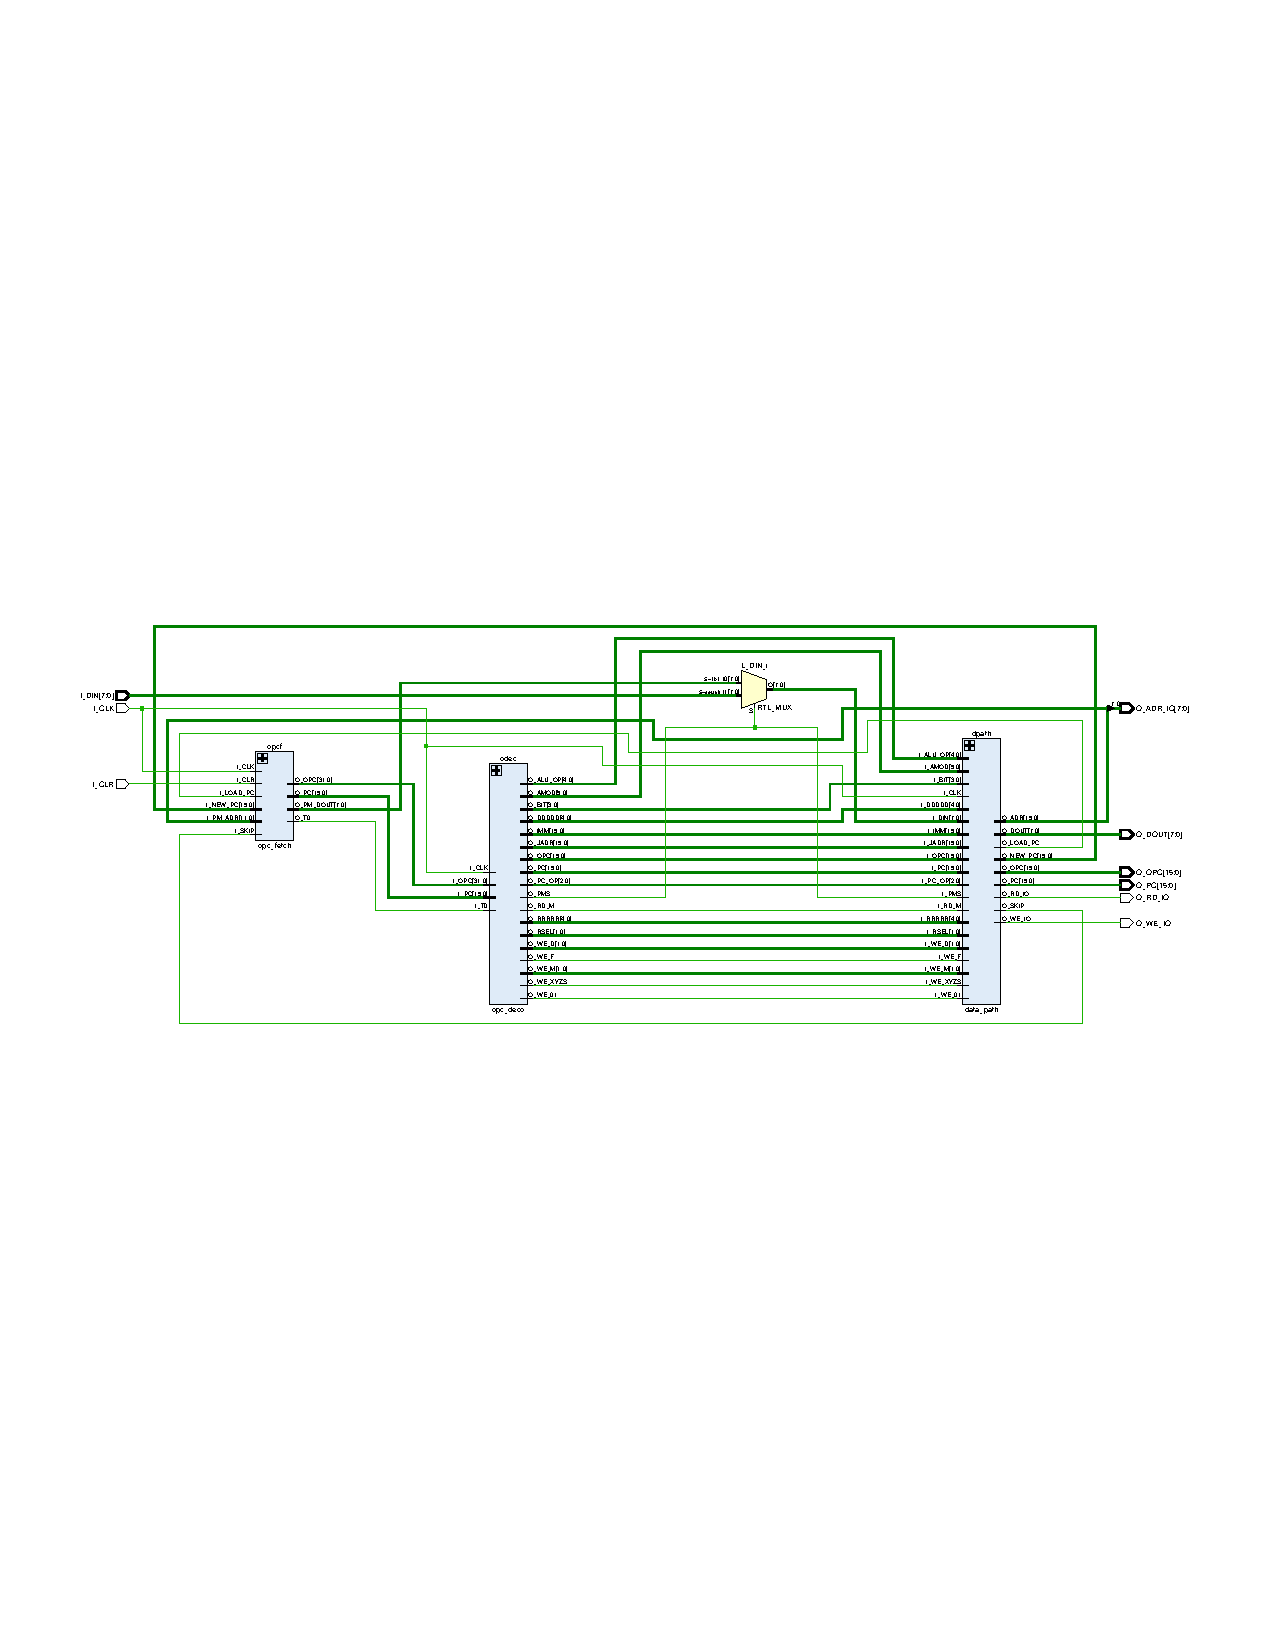
\includepdf[pages={1}]{../schematics/CPU.pdf}
%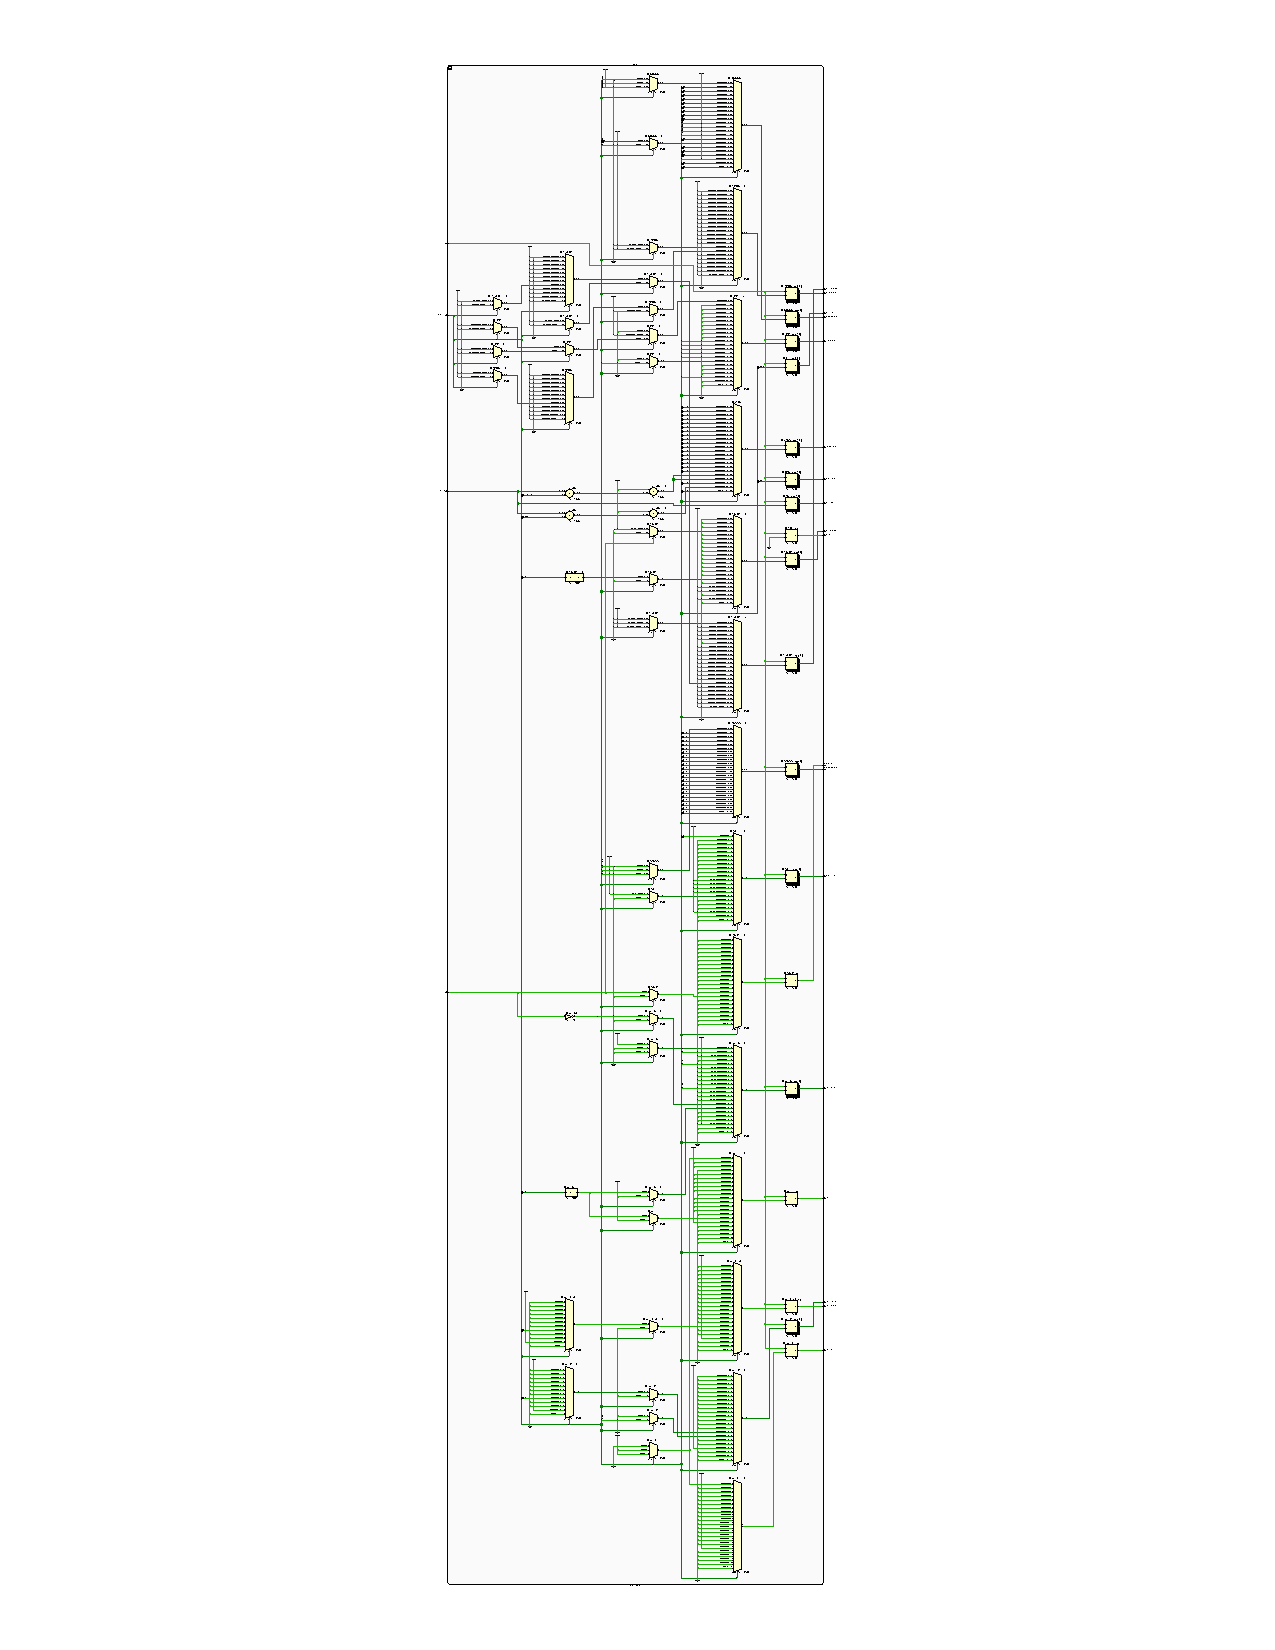
\includepdf[pages={1}]{../schematics/Decoding.pdf}
%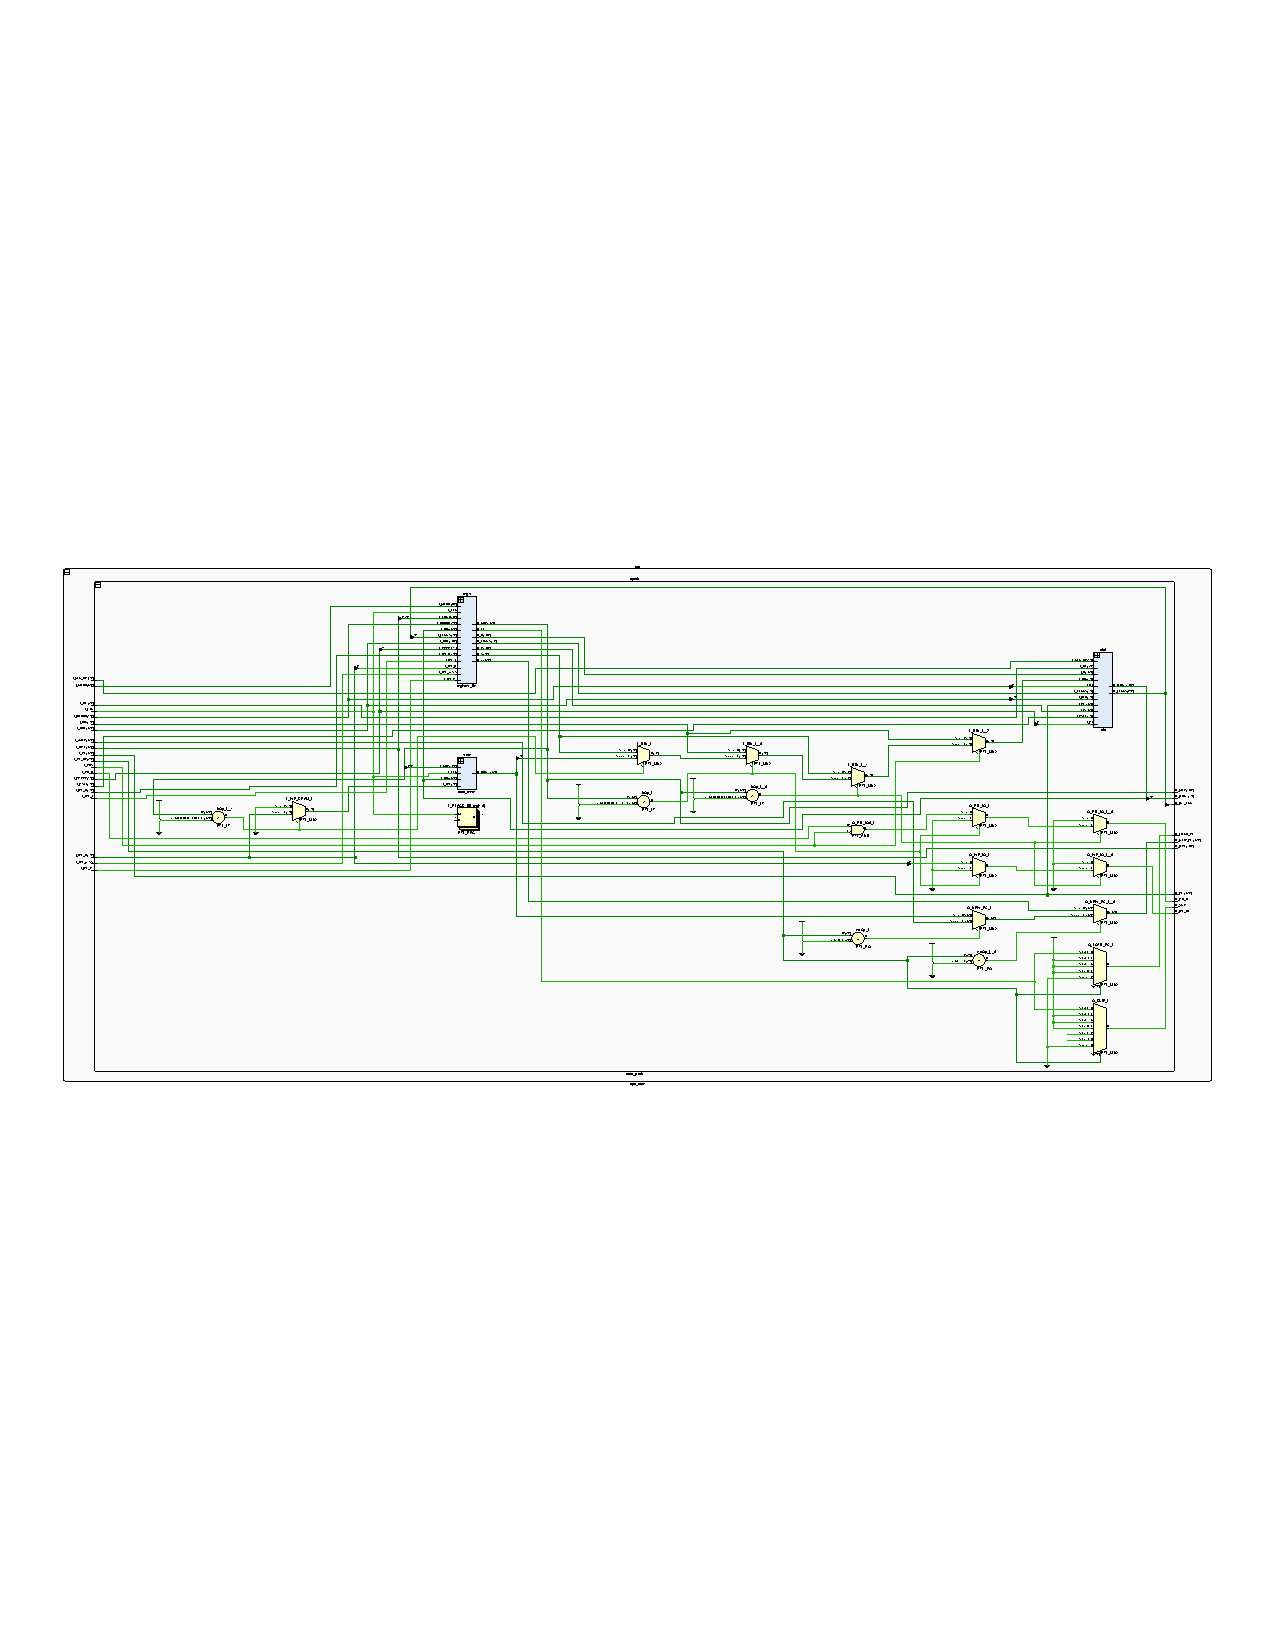
\includepdf[pages={1}]{../schematics/dpath.pdf}

\section{Discussion}
Like the waveform showed in~\ref{fig:waveform}. The general register R24 and R26 is used as a counter. Their initial value is 119. Then both register increase by 1 every 5 clocks. We can see that for the R26, there is one clock in which the value of R26 is different than the value of R24-10. This is caused by the fact that we used two instructions to do this. We first move the R24 to R26, then minus R26-10. So there is one clock in which the value of R26 is different. \\
Though the logic of our processor design is proved. I didn't find a way to do the timing test through a lot of effort. This may be caused by some architecture we use to implement entities. Future work should be done to resolve this problem.\\
\section{Conclusion}
In this project, we designed a basic pipelined CPU. The word ``basic'' is used here because we only designed the CPU core, not including peripheral circuit, so it can't be applied in practical. However, once the CPU core has been designed, the peripheral circuit is very easy to add.\\
The main features of our pipelined CPU including:
\begin{enumerate}
  \item Using dual port memory to solve the structural hazards.
  \item The architecture make it possible that register file and data memory is located in the same stage (executing stage). Thus data hazards are avoided.
  \item A SKIP signal connect the executing stage and opcode fetching stage, which affects the opcode output immediately.
  \item Quite large set of actual instruction is implemented.
\end{enumerate}
Future work including:
\begin{enumerate}
  \item Implement more instructions.
  \item Test with real programs generated by compiler.
  \item Design peripheral circuit.
\end{enumerate}
\end{document}
